\documentclass{article}
\usepackage[utf8]{inputenc}

%\title{}
\title{%
  A qualitative comparison study between \\  
  common GPGPU frameworks. \\
  \large Planning Report, Rev 0.1 \\
}
\author{
    Adam Söderström 930327-3750 \\
    adaso578@student.liu.se 
}
\date{January 2018}

\usepackage{natbib}
\usepackage{graphicx}
\usepackage{rotating}
\usepackage{subcaption}

\begin{document}
\maketitle

\section{Background}
The performance inclination of single-cored CPU's have during the last decades slowly started to decline. The main reason for this declination is due to three "walls":

\begin{itemize}
    \item Instruction Level parallelism wall --- not enough instruction level parallelism to keep the CPU busy
    \item Memory wall --- gap between the CPU speed and off-chip memory
    \item Power wall --- Increased clock rate needs more power which leads to heat problems
\end{itemize}

\noindent This has started a trend where Central Processing Unit (CPU) manufactures have started to create chips containing multiple cores that are run in parallel, see figure \ref{fig:cpuStats}. Today modern CPU's may contain as much as 24 cores, and the number of cores available on a chip seem to be increasing. This technology is however already in use in Graphical Processing Units (GPU), which may contain hundreds of cores. This in turn have spawned a new trend among developers to not just use the GPU to render graphics to the screen, but to perform more general computations. The term used for this is General-purpose computing on graphics processing units (GPGPU).

\begin{figure}[!h]
    \centering
    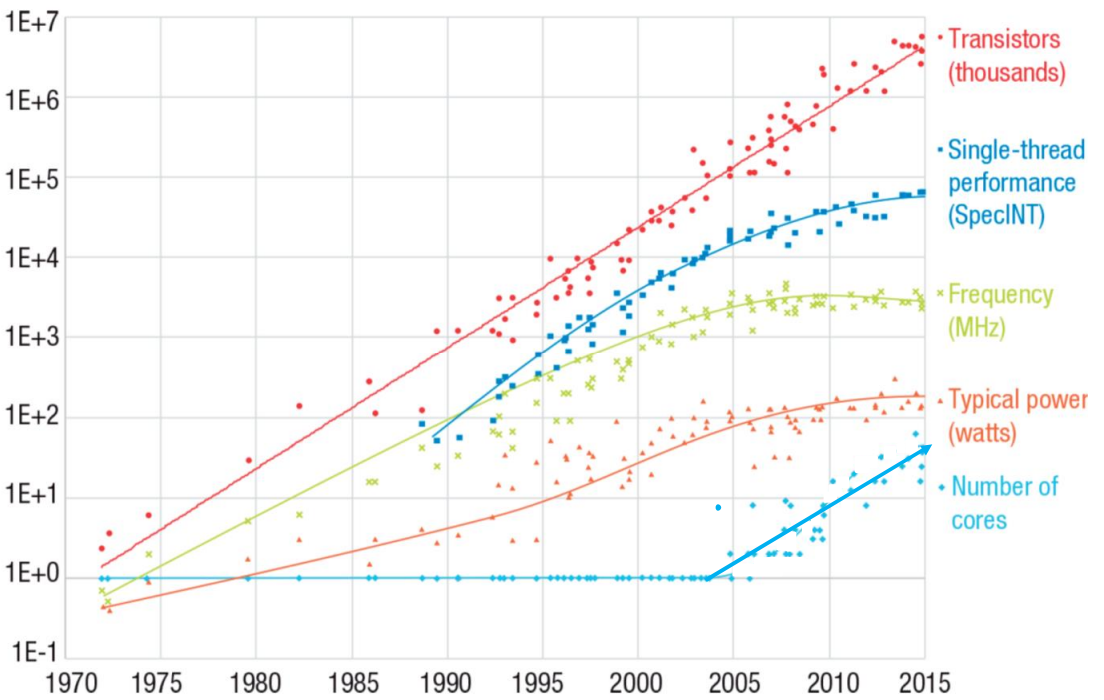
\includegraphics[width=12cm]{Figs/CPUStats.png}
    \caption{Statistics of development for CPU's. \cite{CPUStats}}
    \label{fig:cpuStats}
\end{figure}

In 2007, Nvidia released their framework called CUDA which was developed specifically for GPGPU. Since then, more frameworks and platforms have emerged, most noticeably Open Computing Language (OpenCL), OpenGL Compute Shaders and Microsoft's version of compute shaders for DirectX, DirectCompute. This thesis will focus on evaluating GPGPU frameworks when running a suitable algorithm. Performance, portability and features will be evaluated with focus on the performance. The thesis will be performed at the company MindRoad AB.

\subsection{Algorithm}
This section will discuss algorithms that are candidates for implementation and evaluation. A short description of the algorithm will be presented along with why the algorithm is suitable for a bench-marking application.

\subsubsection{N-body}
An N-Body simulation is an interesting implementation that can be well parallelized. A $N$ number of bodies are simulated where each body is affected by forces from all other bodies. The traditional implementation does thus run in the time complexity $O(n^2)$ but can be further optimized by using the Barnes-Hut algorithm which uses an quad/octree the reduce the time complexity to $O(n \ log \ n)$ \cite{barnes1986hierarchical}. An N-body simulation is often used in traditional GPU bench-marking tests, and it would be interesting to investigate this further when implemented using a GPGPU approach. The bench-marking can be performed in multiple ways; in a real-time simulation and compare the frames-per-second (FPS) with the size of N. In a pre-computed simulation for a fixed amount of time-steps $t_n$, the bench-marking can be performed by comparing the computation time for the entire time-space.


\subsubsection{Parallel Quick-Sort}
The quick-sort algorithm is one of the most popular sorting algorithms. The sorting algorithm runs in the time complexity  $O(n \ log \ n)$ in average, and in the worst case  $O(n^2)$. Although a very popular sequential algorithm, it is not as popular in parallel applications due to its data dependent reorganization. Some research has been done on the subject though and parallel implementations exists \cite{sanders1997efficient}\cite{tsigas2003simple}\cite{manca2016cuda}. The bench-marking in this algorithm can be done by comparing the time consumption when sorting the same input data for all relevant frameworks.

\subsubsection{Anti Aliasing using an Euclidean distance transform function}
A problem in computer graphics is the inability to render sharp surface features when rendered up close, sharp edges in textures often appear jagged when rendered up close. In 2007, Chris Green of Valve Software published a method of dealing with this problem by generating a distance function for a binary image \cite{green2007improved}. An example of C. Green's method applied to a  alpha-blended texture can be seen in figure \ref{fig:valve} \cite{green2007improved}. S. Gustavson et. al. later released an improved version of C. Green's idea, which uses an euclidean distance transform (DT) \cite{gustavson2011anti}\cite{gustavson20122d}. 


\begin{figure}[!h]
    \centering
    \begin{subfigure}[b]{0.271\textwidth}
        
\includegraphics[width=\textwidth]{Figs/ValveAlphaBlended.png}
        \caption{64x64 texture, alpha-blended}
        \label{fig:valveA}
    \end{subfigure}
    ~
    \begin{subfigure}[b]{0.3\textwidth}
        
\includegraphics[width=\textwidth]{Figs/ValveAlphaTested.png}
        \caption{64x64 texture, alpha tested}
        \label{fig:valveA}
    \end{subfigure}
    ~ 
    \begin{subfigure}[b]{0.3\textwidth}
        
\includegraphics[width=\textwidth]{Figs/ValveGreensTechnique.png}
        \caption{64x64 texture using Green's technique}
        \label{fig:mouse}
    \end{subfigure}
    \caption{Vector art encoded in a 64x64 texture using (a) simple bilinear filtering (b) alpha testing and (c) Green's distance field technique}\label{fig:animals}
    \label{fig:valve}
\end{figure}

V. Ilic et. al. later extended this into three-dimensions using a similar DT technique based on C. Green's technique \cite{ilic2015precise}. 

The algorithm works on pixel level and is thus very well suitable for parallelization. It is also easy to use this algorithm for a bench-mark application by comparing the time consumption when running the algorithm on the different frameworks.


\section{Problem formulation}
\begin{itemize}
    \item What is a suitable bench-marking algorithm?
    \item What factors can be compared more than the execution time?
    \item How does a parallel implementation compare to a sequential implementation?
\end{itemize}


\section{Approach}
The report will be written in parallel with the implementation and will written according to the Gantt-chart presented in figure \ref{fig:GanttChart}. The Gantt-chart also specifies more precise time approximations and scheduling.

At the end of each week a short summary describing the work performed will be submitted to the examiner and to MindRoad AB.

\begin{itemize}
    \item Explore previous comparisons/bench-marks between CUDA, OpenCL and DirectCompute. 
    \item Investigate the algorithm and find parts that can be parallelized.
    \item Examine previous research on the subject.
    \item Investigate useful technologies that can be used in the implementation.
    \item Implement a simple "Hello World" application in all environments.
    \item Develop a sequential implementation used for comparison.
    \item Implement a CUDA application running the algorithm, perform necessary optimization's.
    \item Port the CUDA implementation to OpenCL and DirectCompute.
    \item Perform measurements between the different implementations.
\end{itemize}


\begin{sidewaysfigure}[!h]
    \centering
    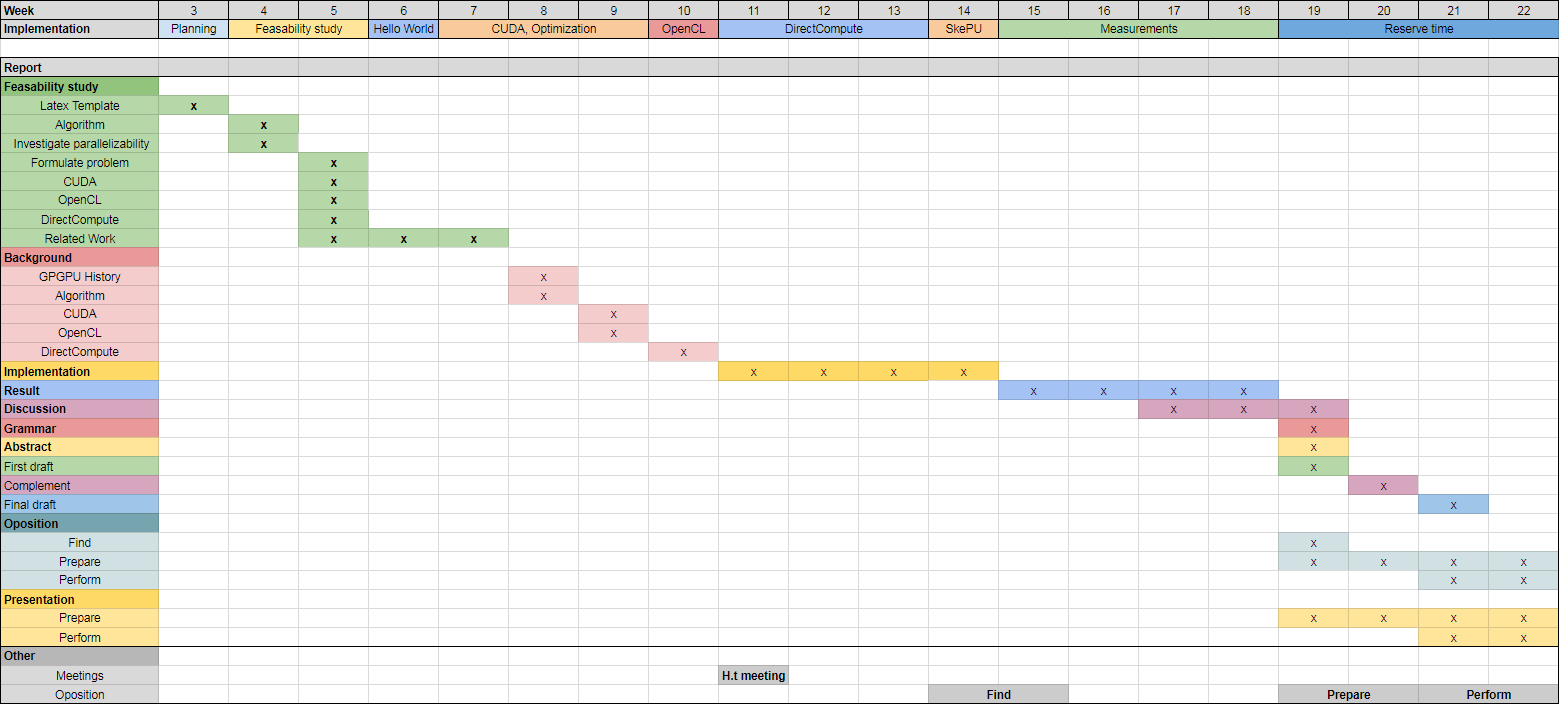
\includegraphics[width=1.1\textwidth]{Figs/Gantt-chart.png}
    \caption{Detailed Gantt-chart describing the implementation and report work-flow}
    \label{fig:GanttChart}
\end{sidewaysfigure}




\section{Delimitations}
This section will present some delimitations for the implementation, both in terms of the GPGPU implementation, as well as some limitations of the selected algorithm.

\subsection{GPGPU}
The selected algorithm will only be implemented in the discussed frameworks:
\begin{itemize}
    \item CUDA
    \item OpenCL
    \item DirectCompute
\end{itemize}

\noindent aswell as a traditional implementation. The selected algorithm will thus not be implemented in other GPGPU frameworks such as OpenGL's compute shader, or a parallel CPU based implementation, using e.g OpenMP or similar frameworks.

\subsection{N-Body}

\subsection{Parallel Quick Sort}

\subsection{Anti-Aliasing using an Euclidean distance transform function}
Although a three-dimensional extention exists to C. Green's method \cite{green2007improved}, the implementation will only be performed in 2D using S. Gustavsons improved version of the technique \cite{gustavson2011anti}.

\section{Resources}
The resources listed below will be used regardless of what algorithm is selected. Additinal resources such as OpenGL will be used if a visualization based algorithm is chosen.

\begin{itemize}
    \item CUDA - http://docs.nvidia.com/cuda/
    \item OpenCL - https://www.khronos.org/opencl/
    \item DirectCompute - https://msdn.microsoft.com/en-us/library/windows/desktop/ff476331(v=vs.85).aspx
    \item Course material from the course TDDD56 - Multicore and GPU Programming 
\end{itemize}


\bibliographystyle{plain}
\bibliography{references}

\end{document}
